\newcommand{\stencilpt}[4][]{\node[draw,inner sep=0.1em,minimum size=1.2cm,font=\small,#1] at (#2) (#3) {#4}}
\begin{frame}{Stencil}   
    \centering
    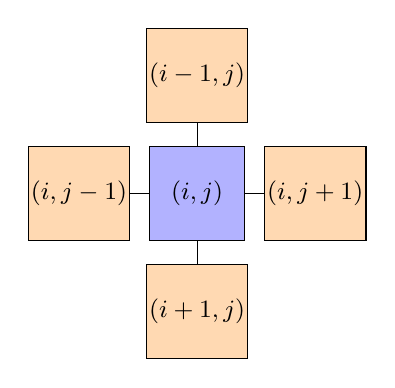
\begin{tikzpicture}
      \stencilpt[fill=orange!30]{-1.5,0}{i-1}{$(i, j-1)$}; % Left neighbor
      \stencilpt[fill=blue!30]{0,0}{i}{$(i, j)$}; % Central point
      \stencilpt[fill=orange!30]{1.5,0}{i+1}{$(i, j+1)$}; % Right neighbor
      \stencilpt[fill=orange!30]{0,1.5}{j+1}{$(i-1, j)$}; % Top neighbor
      \stencilpt[fill=orange!30]{0,-1.5}{j-1}{$(i+1, j)$}; % Bottom neighbor
    
      \draw (i) -- (i-1)
            (i) -- (i+1)
            (i) -- (j+1)
            (i) -- (j-1);
    \end{tikzpicture}
\end{frame}
